% tutorial.tex  -  a short descriptive example of a LaTeX document
%
% For additional information see  Tim Love's ``Text Processing using LaTeX''
% http://www-h.eng.cam.ac.uk/help/tpl/textprocessing/
%
% You may also post questions to the newsgroup <b> comp.text.tex </b> 

\documentclass[12pt]{article}			% For LaTeX 2e
						% other documentclass options:
						% draft, fleqn, openbib, 12pt

\usepackage{graphicx}	 			% insert PostScript figures
%% \usepackage{setspace}   % controllabel line spacing
%% If an increased spacing different from one-and-a-half or double spacing is
%% required then the spacing environment can be used.  The spacing environment 
%% takes one argument which is the baselinestretch to use,
%%         e.g., \begin{spacing}{2.5}  ...  \end{spacing}


% the following produces 1 inch margins all around with no header or footer
\topmargin	=10.mm		% beyond 25.mm
\oddsidemargin	=0.mm		% beyond 25.mm
\evensidemargin	=0.mm		% beyond 25.mm
\headheight	=0.mm
\headsep	=0.mm
\textheight	=220.mm
\textwidth	=165.mm
					% SOME USEFUL OPTIONS:
% \pagestyle{empty}			% no page numbers
 \parindent  15.mm			% indent paragraph by this much
 \parskip     2.mm			% space between paragraphs
% \mathindent 20.mm			% indent math equations by this much

\newcommand{\MyTabs}{ \hspace*{25.mm} \= \hspace*{25.mm} \= \hspace*{25.mm} \= \hspace*{25.mm} \= \hspace*{25.mm} \= \hspace*{25.mm} \kill }

\graphicspath{{../Figures/}{../data/:}}  % post-script figures here or in /.

					% Helps LaTeX put figures where YOU want
 \renewcommand{\topfraction}{0.9}	% 90% of page top can be a float
 \renewcommand{\bottomfraction}{0.9}	% 90% of page bottom can be a float
 \renewcommand{\textfraction}{0.1}	% only 10% of page must to be text

\linespread{1.2}
\alph{footnote}				% make title footnotes alpha-numeric

\title{Continuous Authentication\\using video-based face recognition}	% the document title
\author{{\bf Project report - Phase I}{\bf}}
\date{}				% your own text, a date, or \today

% --------------------- end of the preamble ---------------------------

\begin{document}			% REQUIRED

\pagenumbering{roman}			% Roman numerals from abstract to text
\maketitle				% you need to define \title{..}
\thispagestyle{empty}			% no page number on THIS page 

\begin{center}

%A synopsis submitted in partial fulfillment of the requirements of the course \\[3ex]
{\Large CS812}\\[3ex]
{\Large}

{\large}
{\bf Under the guidance of }{\bf}\\[2ex]
Dr. K. G. Srinivasa\\
Professor\\
Department of Computer Science and Engineering\\
M. S. Ramaiah Institute of Technology\\[3ex]


{\bf Submitted by}{\bf}\\[2ex]
{\bf Soumya Gosukonda }{\bf} 1MS08CS119\\
{\bf Tribhuvanesh Orekondy }{\bf} 1MS08CS129\\[8ex]
{\large}


\includegraphics[scale=0.20]{msrit.png}\\
Department of Computer Science and Engineering\\
M. S. Ramaiah Institute of Technology\\
(Autonomous Institute Affiliated to VTU)\\
Bangalore - 560054
\end{center}

\newpage
\begin{abstract}			% beginning of the abstract

% TODO <-----ABSTRACT GOES HERE------>

Password based security is a commonly used measure to enforce valid authentication. Coupled with Iris and/or fingerprint based recognition, these systems, known as biometric authentication systems, strengthen this process of authentication. However, this is a one-time process and fails to provide continuous authentication. To illustrate the idea of Continuous Authentication (CA) consider a situation where the user has to leave her/his workstation unattended for a short period of time and forgets to lock it. In this time interval it is possible for an unauthorized user to gain access to the system and tamper with it. To avoid such a situation, continuous authentication can prove useful. 
This project aims to deliver a continuous authentication system based on face recognition and soft biometric traits, namely shirt colour. We plan to achieve this goal using the OpenCV library and a suitable mathematical model.


\end{abstract}				% end of the abstract

\newpage				% start a new page
\tableofcontents			% create table of contents automatically
\newpage				% start a new page
\pagenumbering{arabic}			% Arabic page numbers from now on

\section{ Introduction }	% start the first numbered section

% <-------- INTRODUCTION -------->

\subsection{ General Introduction }
Static Authentication enables a user to log in to a session through his/her account by providing the required credentials at the beginning. This form of authentication doesn’t consider the possibility of tailgating when the authorized user is not present in front of the authenticated system. On the other hand, Continuous Authentication provides a solution by authenticating the user right from the initial stages of log-in through log-out. This is implemented by checking the facial features of the user during log in, followed by creating a template of the user containing his/her soft biometric traits, which in this case, is the colour of the user’s clothing [Niinuma et al]. 

\subsection{ Problem Definition }
Soft biometric traits don’t provide as high a level of confidence when compared to hard biometric traits. The problem here is to design a system by which the threshold of confidence in authenticating the user can be increased by intelligently verifying these hard biometric traits by implementing a suitable machine learning algorithm.


\section{Literature Survey }
%\subsection{ Continuous Authentication }


\subsection{ OpenCV }
OpenCV (Open Source Computer Vision Library) is a library of programming functions mainly aimed at real time computer vision, developed by Intel and now supported by Willow Garage. It is free for use under the open source BSD license. The library is cross-platform. It focuses mainly on real-time image processing. If the library finds Intel's Integrated Performance Primitives on the system, it will use these proprietary optimized routines to accelerate itself.

\subsection{ Face Detection }
OpenCV's face detector uses a method that Paul Viola and Michael Jones published in 2001 [1]. Usually called simply the Viola-Jones method, or even just Viola-Jones, this approach to detecting objects in images combines four key concepts:
\begin{itemize}
	\item{} Simple rectangular features, called Haar features
	\item{} An Integral Image for rapid feature detection
	\item{} The AdaBoost machine-learning method
	\item{} A cascaded classifier to combine many features efficiently
\end{itemize}

\subsubsection{ EigenFace }
Eigenface [2] consists of two phases: learning and recognition. In the learning phase, you give eigenface one or more face images for each person you want it to recognize. These images are called the training images. In the recognition phase, when you give eigenface a face image, it responds by telling you which training image is "closest" to the new face image.

Eigenface uses the training images to "learn" a face model. This face model is created by applying a method called Principal Components Analysis (PCA) to reduce the "dimensionality" of these images. Eigenface defines image dimensionality as the number of pixels in an image.

The lower dimensionality representation that eigenface finds during the learning phase is called a subspace. In the recognition phase, it reduces the dimensionality of the input image by "projecting" it onto the subspace it found during learning. "Projecting onto a subspace" means finding the closest point in that subspace. After the unknown face image has been projected, eigenface calculates the distance between it and each training image. Its output is a pointer to the closest training image. You can then look up which person that was to see whom eigenface has identified.

\subsection{ Soft Biometric Traits }
Soft Biometric Traits refers to features of the user that identify the user on a temporary basis [3]. These can refer to, but are not limited to, the following:
\begin{itemize}
	\item{} Physical: colour of skin, eyes and/or hair, presence of beard/moustache.
	\item{} Behavioural: gait, keystrokes.
	\item{} Adhered Human Characteristics: clothes colour, tattoos, accessories such as spectacles.
\end{itemize}

This approach has been well-researched and documented in \textit{Soft Biometric Traits for Continuous User Authentication} by Niinuma et al., Fujitsu Lab, 2010.

\section{Software Requirements Specification }
\subsection{ Introduction }

\subsubsection{ Purpose }
The purpose of this Software Requirements Specification is to provide a complete description of all the specifications and functions of the Continuous Authentication system as described above.

\subsubsection{ Scope of the Project }
Continuous authentication prevents the system from compromising the user's authenticity by continuously ensuring that the confidence in the identity of the user doesn't fall below a certain threshold. A video-feed from the web-cam is used to capture the user's traits throughout the session. A session here can be associated with the user logged-in to an e-mail or online banking account, or an account on the operating system itself.

\subsubsection{ Overview of Document }
The rest of this Software Requirements Specification proceeds with a general description of the project followed by the specific requirements of this software. 

\subsection{ General Description }
\subsubsection{ Project Perspective }
The Continuous Authentication system is designed as a stand-alone application which grants the user certain privileges at the time of successful log-in and continuously authenticates the user. The application enters into a lock-down mode in case an unauthorized  user attempts to use the authenticated user's privileges. 

\subsubsection{ Product Functions }
The Continuous Authentication system aims to provide the two primary functions:
\begin{itemize}
	\item To check the hard biometric traits of the user during the initial log-in stage and during certain periods after log-in till session ends.
	\item Continuously monitor the identity of the authenticated user and lock-down when required.
\end{itemize}

\subsubsection{ End users }
This application provides an added layer of security for users who wish to protect access to confidential information. Consequently, the user can rely on the system to ensure the privacy of his/her information.

\subsubsection{ General Constraints }
This application is constrained by the following:
\begin{itemize}
	\item The end-user's system should be capable of processing the real-time video-feed.
	\item The lighting conditions during usage to be similar to that captured by the training set.
	\item The system is incapable of performing a hard biometric recognition in case of occlusion.
\end{itemize}

\subsubsection{ Assumptions and Dependencies }
This application is assumes the following:
\begin{itemize}
	\item The user's system is equipped with a web-cam.
	\item The user is working in a sufficiently illuminated environment.
\end{itemize}

\subsection{ Specific Requirements }
\subsubsection{ Functional Requirements }
\begin{itemize}
	\item{\it Provide initial log-in, and verify user's password followed by the user's hard biometric traits. }
	\item{\it Create an account for a new user in the xml database and collect user's facial features and retrain the model. }
	\item{\it Create a user template with the user's soft biometric traits (shirt colour) once the user's face has been recognized with a minimum given confidence level.  }
	\item{\it Use the shirt-colour template to continuously verify the user's identity.  }
	\item{\it If the soft biometric verification falls below a certain threshold, restart face recognition of the user.  }
	\item{\it Lock-down in case of a tailgating unauthorized user. }
	%\item{\it A session time-out occurs in case the user logs in and then leaves the workstation unattended for a specified time limit. }
\end{itemize}

\subsubsection{ Software Requirements }
\begin{itemize}
\item C++ compiler (g++ 4.6.1)
\item OpenCV libraries
\item Drivers for web-cam
\item Python 2.7.1
\end{itemize}

\subsubsection{ Hardware Requirements }
\begin{itemize}
\item Web-cam with drivers supported by OpenCV, with a minimum resolution of 1.3MP
\item Memory : 2GB DDR2
\item Processor : A minimum of 3.0GhZ single core processor
\end{itemize}

\subsection{ Interface Requirements }
\subsubsection{ User Interface }
The user interface is provided with functions necessary to take as input the credentials of the user and display the live video-feed from the web-cam.

\section{ System Architecture and Design }  
\subsection{ Block diagram }
\begin{center}
    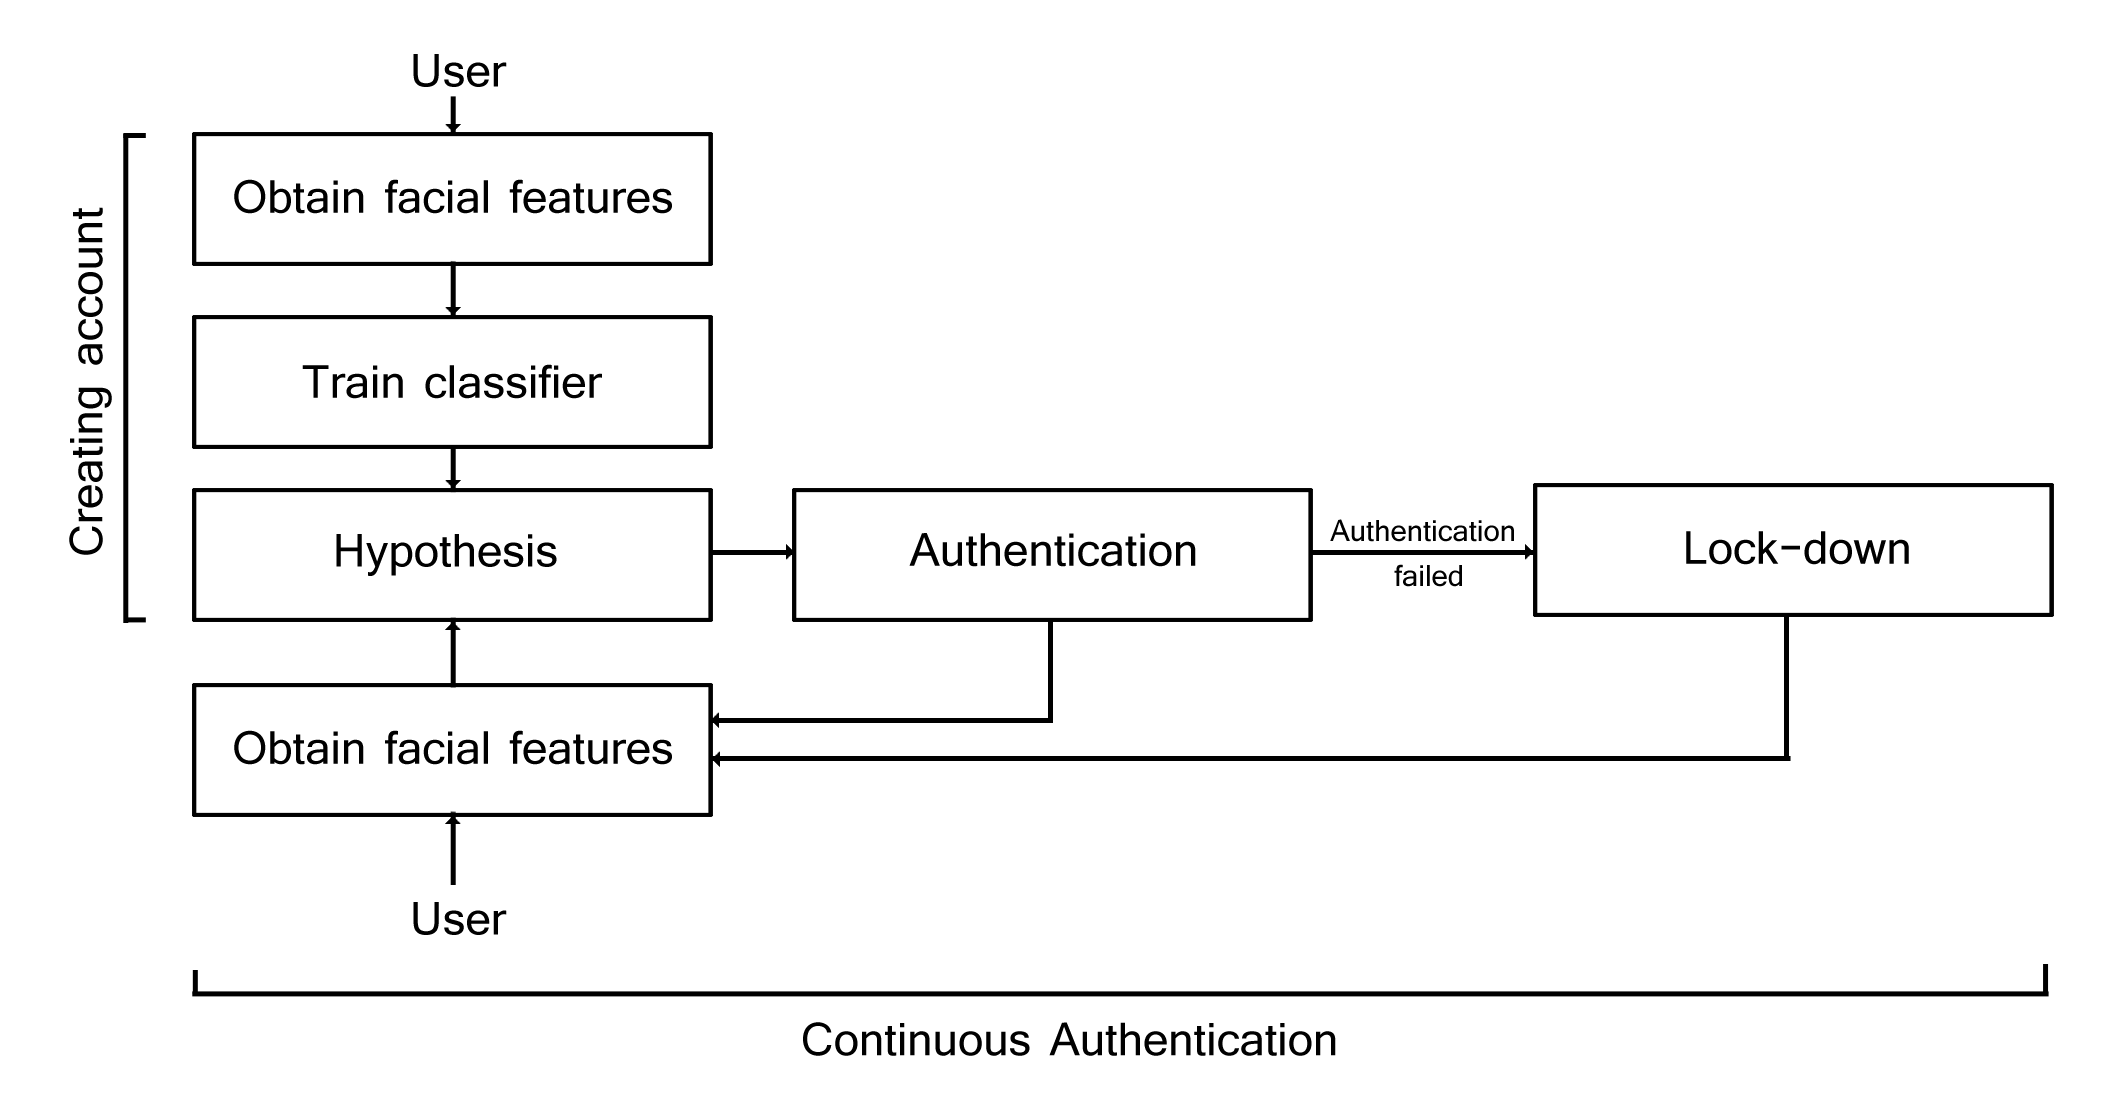
\includegraphics[scale=0.8]{block.png}
\end{center}

\section{ Detailed Design }
\subsection{ Data Description }
The data of the system can be divided into the following parts:
\subsubsection{ Account and Face Data }
  

\section{ Implementation }  

\section{ Testing }

\section{ Conclusion and Future Enhancements }

\section{ References }
[1] Paul Viola, Michael Jones. Robust Real-time Object Detection. \textit {Second International Workshop on Statistical and Computational Theories of Vision - Modeling, Learning, Computing, and Sampling} (Vancouver, Canada), July 13, 2001. 

[2] Matthew Turk, Alex Pentland. Eigenfaces for Recognition. \textit {Journal of Cognitive Neuroscience} (Massachusetts Institute of Technology), 1991. 

[3] A.K. Jain, S.C. Dass, K. Nandakumar. Soft biometric traits for personal recognition systems. \textit{ International Conference on Biometric Authentication.} 2004.
 
[4] Niinuma et al. Soft Biometric Traits for Continuous User Authentication. \textit{Fujitsu Lab}. 2010.

\section{ Appendix }
\subsection{ Screen Snapshots}

% \section{ Applications }  
\end{document}				% REQUIRED

